\section{Methods}
\label{sec:Methodes}
\begin{frame}{Optimization Formulation}
The optimization of the films was formulated as finding the minimum mass of \iso[6]{Li} for a given detector material necessary to fulfill an interaction rate of \SI{2.5}{cps\per\nano\gram\iso[252]{Cf}} while maintaining a intrinsic gamma rejection ratio of \num{1.e-6}.

It is assumed that there is a fixed cost to assemble each detector assembly and mount it between the moderator.
\end{frame}

\begin{frame}[fragile]{Geometry}
\begin{itemize}
	\item Slices of moderator and assemblies
	\item Each assembly can contain multiple film layers
	\item A compact representation can be obtained \verb+010010+
\end{itemize}
\begin{figure}
    \centering
    \begin{subfigure}[b]{0.45\textwidth}
        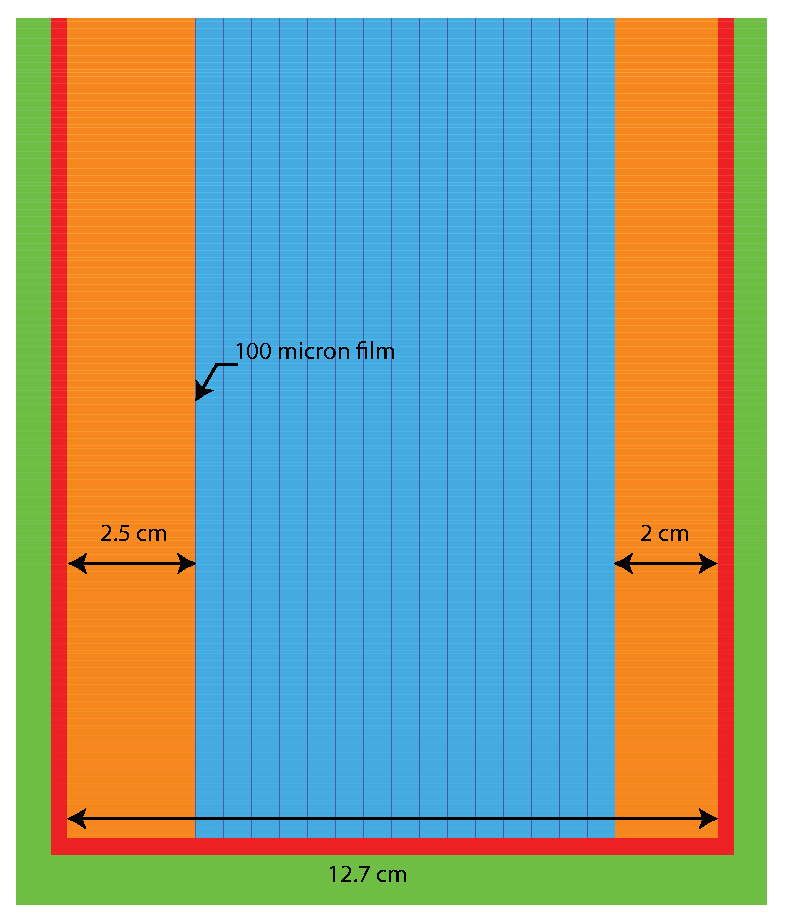
\includegraphics[width=\textwidth]{RPM8_Diagrams_MCNPXRender_1Assm}
        \caption{MCNPX Model of One Assembly}
    \end{subfigure}%
    ~
    \begin{subfigure}[b]{0.45\textwidth}
        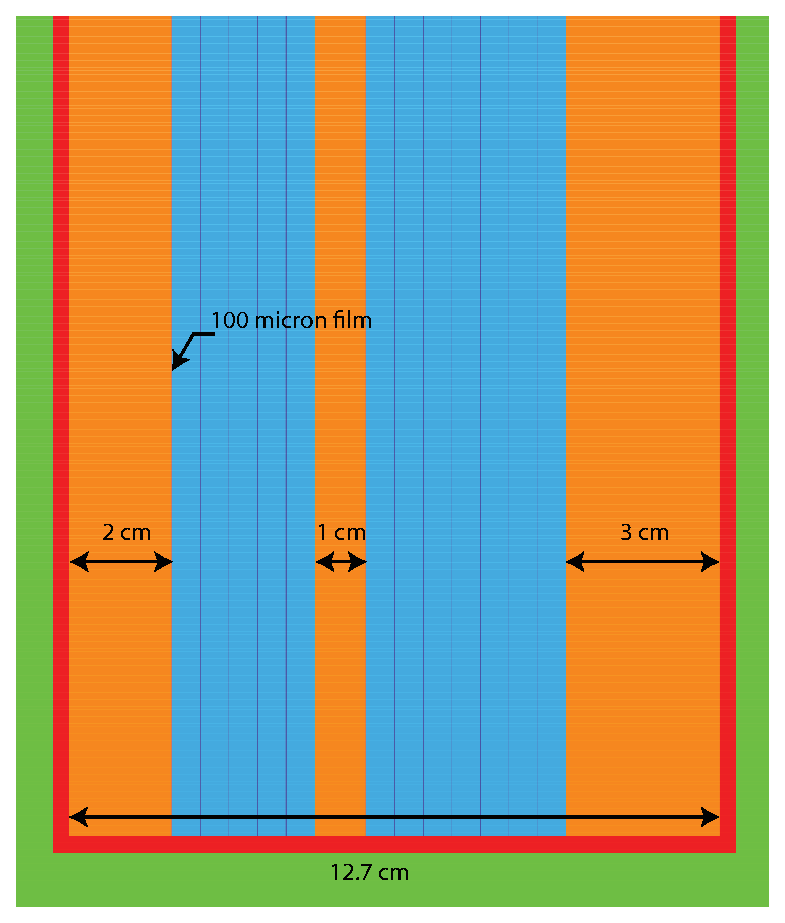
\includegraphics[width=\textwidth]{RPM8_Diagrams_MCNPXRender_2Assm}
        \caption{MCNPX Model of Two Assemblies}
    \end{subfigure}
    \caption{MCNPX rendering of layered geometry}
    \label{fig:MCNPXRendering}
\end{figure}
\end{frame}

\begin{frame}{Genetic Algo}
\begin{figure}
\begin{algorithmic}
  \WHILE{$error>goal$}
		\FORALL{$p \in P$}
			\STATE{Compute fitness}
		\ENDFOR
		\FORALL{$p \in P$}	
			\STATE{Choose individuals based on fitness}
			\STATE{Select individuals for next population}
			\STATE{Crossover selected individuals}
			\STATE{Mutate selected individual}
		\ENDFOR
	\ENDWHILE
\end{algorithmic}
\caption{Genetic Program Outline}
\label{AlgoOutline}
\end{figure}
\end{frame}
\begin{frame}[fragile]{Genome Representation}
The genome representation of the geometry was chosen to be represented as a bit string of a set length.
Each \verb+1+ or \verb+0+ in the string would represent a detector slice or a moderator slice, respectively.
For example the sequence \verb+0001110010+ would represent a detector that had three moderator slices, three detector slices, another two moderator slices, and a final detector slice before a single moderator slice as the reflector.
It was originally thought to have all of the moderator and detector slice the same thickness, \SI{0.5}{\centi \meter}\footnote{Astute readers may note that with a \SI{0.5}{\centi \meter} light guide and \SI{100}{\micro \meter} detector that the detector size is not \SI{0.5}{\centi\meter} and that 25 slices of \SI{0.5}{\centi\meter} each is \SI{0.2}{\centi\meter} short of the RPM8 size. However, it is not envisioned that \SI{20}{\milli\meter} will greatly impact the solution, or be within the manufacturing tolerances. }.
However, that would create 25 slices with a search space of $2^{25}$ or 33.5 million options.
\end{frame}
\begin{frame}{Fitness Function}
The fitness function was choosen to count rate per mass of \iso[6]{Li}, provided that the geometry meet the total count rate criteria.
If it failed to meet the count rate criteria a zero fitness was returned \eqref{eqn:FitnessFun}.
\begin{align}
    \label{eqn:FitnessFun}
    f(\vec{x})
    = \begin{cases}
    0 & \text{if} \text{countRate}(\vec{x}) \leq \SI{2.5}{cps\per\nano\gram\iso[252]{Cf}} \\
    \text{countRatePerMass}(\vec{x})
    \end{cases}
\end{align}
\end{frame}
\begin{frame}[fragile]{Mutation, Crossover and Selection}
The mutation operation was chosen to be a simple bit flip in which a randomly chosen \verb+1+ or \verb+0+ in the geoemtry was flipped; for example \verb+001001010+ could be mutated to \verb+001001000+.
Crossover, in which two individuals are breed in produce the new generataion was implemented as \textbf{VALUE}.
The pyevolve toolkit was used for running of the genetic algorthim.
The genetic algorthim used a mutation rate of 2\% and a crossover rate of 80\%
Tournamnet selectrion was used to determine which individuals would be allowed to breed for the next generation.
\end{frame}
\begin{frame}{Computional Size}
\begin{table}
    \caption[Genome Bit String Geometries]{Bit String Simplified Geometetry Descriptions}
    \label{tab:BitStringGeo}
    \centering
    \begin{tabular}{ c | c c c c}
        Genome Length&Films Per Assembly&Slice Thickness&Light Guide Thickness&Possible Geomeries \\
        \hline
        \hline
        3&4&4.23&1.058&7 \\
        4&4&3.18&0.794&15 \\
        5&3&2.54&0.847&31 \\
        6&3&2.12&0.706&63 \\
        7&3&1.81&0.605&127 \\ 
        \hline
        10&3&1.27&0.423&1023 \\
        \hline
        13&2&0.98&0.488&8191 \\
        26&1&0.49&0.488&67108863 \\
    \end{tabular}
\end{table}
\end{frame}


